\documentclass[a4paper,11pt]{article}
\usepackage[utf8]{inputenc}
\usepackage{minted}
\usepackage{amsmath}
\usepackage{float}
\usepackage{footmisc}
\usepackage{graphicx}
\usepackage{multirow}
\usepackage[toc,page]{appendix}

\graphicspath{{./figures/}}

\title{\textbf{11. T9}}
\author{Kristiāns Vinters}
\date{Fall 2023}

\begin{document}
    \maketitle
    \section*{Introduction}

    I solved the assignment in Go. I used Go because I want to become more familiar with it. Source code and benchmark data is available on GitHub\footnote{https://github.com/Phanty133/id1021/tree/master/11-trie}.

    \section*{Implementation}

    I implemented the trie in a single file, \texttt{trie.go}. I implemented the \texttt{GetCharCode()} and \texttt{GetCharFromCode()} functions with a shorter approach than was suggested in the assignment. I used special cases for the swedish characters, but used one general case for ASCII characters and skipped \texttt{q} and \texttt{w} with index increments/decrements.

    \begin{minted}{go}
// GetCharFromCode() is basically the same,
// but does the inverse and returns a rune instead of an int.
func GetCharCode(char rune) int {
    switch char {
    case 'å':
        return 24
    case 'ä':
        return 25
    case 'ö':
        return 26
    default:
        if char >= 'q' {
            char -= 1
        }

        if char >= 'w' {
            char -= 1
        }

        return int(char) - 'a'
    }
}
    \end{minted}

    The \texttt{getIdx()} function is implemented with a similar approach by subtracting ASCII code values:

    \begin{minted}{go}
func getIdx(key rune) int {
    return int(key-'0') - 1
}
    \end{minted}

    The \texttt{AddWord()} function is implemented with a loop.

    \begin{minted}{go}
func (t *Trie) AddWord(word string) {
    curr := t.root

    for _, char := range word {
        idx := GetCharCode(char)

        if curr.next[idx] == nil {
            curr.next[idx] = NewNode()
        }

        curr = curr.next[idx]
    }

    curr.valid = true
}
    \end{minted}

    Lookup is implemented recursively. There's an initial \texttt{Trie.Lookup()} function call that executes a \texttt{TrieNode.Lookup()} function on the root node. It uses a path that gets updated and a pointer to a string array to which the results are appended.

    \begin{minted}{go}
func (t *Trie) Lookup(seq string) []string {
    output := make([]string, 0)
    t.root.Lookup(seq, "", &output)

    return output
}

func (t *Node) Lookup(seq string, path string, output *[]string) {
    // Terminating case, which finalizes the word.
    // If the word appears in the dataset, it is appended to the output array.
    if len(seq) == 0 {
        if t.valid {
            *output = append(*output, path)
        }

        return
    }

    // Convert sequence digit to an array of possible branch array indices.
    idx := getBranchIdxesFromKey(rune(seq[0]))

    // Iterate over each branch index and execute Lookup() on all non-nil nodes.
    for _, i := range idx {
        if t.next[i] != nil {
            t.next[i].Lookup(seq[1:], path+string(GetCharFromCode(i)), output)
        }
    }
}
    \end{minted}

    \section*{Statistics}

    For every word in the dataset, I measured how many words you'd be suggested if you were trying to type that word. While analyzing the dataset, I also found out that the \texttt{kelly.txt} file contains word duplicates, which I had to filter out for the statistics to make sense. The largest set is 7 words, of which there are two. There is no 6 word set, but there is a single 5 word set.
    
    \begin{figure}[H]
        \centering
        
        \begin{tabular}{c|c}
            \textbf{Suggested \#} & \textbf{Words} \\
            \hline
            \hline
            \multirow{14}{*}{7} & lås \\
            & kår \\
            & kör \\
            & kär \\
            & lös \\
            & lår \\
            & köp \\
            \cline{2-2}
            & läsa \\
            & köpa \\
            & låsa \\
            & löpa \\
            & köra \\
            & lära \\
            & lösa \\
            \hline
            \multirow{5}{*}{5} & röka \\
            & söka \\
            & röja \\
            & råka \\
            & räka \\
        \end{tabular}
        \caption{Suggested word sets}
        \label{fig:lookup-table}
    \end{figure}

    \begin{figure}[H]
        \centering
        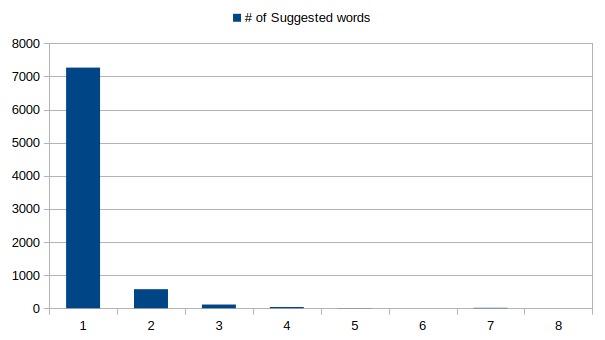
\includegraphics[width=\textwidth]{duplicates.png}
        \caption{Suggested word count histogram}
        \label{fig:duplicates}
    \end{figure}

    \begin{figure}[H]
        \centering
        
        \begin{tabular}{c|c}
            \textbf{Suggested \#} & \textbf{Count} \\
            \hline
            \hline
            1 & 7268 \\
            2 & 574 \\
            3 & 111 \\
            4 & 36 \\
            5 & 5 \\
            6 & 0 \\
            7 & 14 \\
        \end{tabular}
        \caption{Suggested word counts}
        \label{fig:duplicates-table}
    \end{figure}
\end{document}
